\chapter{Results}
\label{results}

This chapter will cover the results of the best and final model that was trained.  The first section, \nameref{evaluation}, measures the performance
of piece recognition against existing solutions.  The second section, \nameref{evaluate pgn}, tests the model within the inference application
to give a better view of its utility.

\section{Piece Recognition}
\label{evaluation}

The best openly available solutions for chess piece recognition were found and trained on the chessboard used throughout this project.
As can be seen, the presented solution outperformed the others by a huge margin, despite using data from the evaluation set that had never
been used to train the presented model.  In order to make a fairer comparison another board entirely was also chosen for these final tests.  The 
reason being that it is more than possible through each iteration and optimisation of hyperparameters the presented solution was being overfit to the 
images in the evaluation set despite never being directly trained on it.  By now including a never seen before dataset more meaningful conclusions
regarding the generality of the model can be drawn.

Use top-1 and top-5 to measure performance of different models.
Will include basic evaluation.  What happens what you increase layers, use more data, data augmentation.
Include Recall / Specificity / Sensitivity



Using a neural network instead as an additional class with our piece recognition network.
Compare that two having a two stage network, the first for piece detection and the second for recognition.

\begin{center}
    \begin{tabular}{|c|c|c|c|c|c|c|}
        \cline{2-7}
        \multicolumn{1}{c|}{} & \multicolumn{3}{|c|}{Chessboard 1} & \multicolumn{3}{|c|}{Chessboard 2} \\
        \hline
        Method & Accuracy & Precision & Recall & Accuracy & Precision & Recall \\
        \hline
        proposed & \textbf{94\%} & 1 & 2 & 3 & 4 & 4 \\
        \cite{} & 78\% & 1 & 2 & 3 & 4 & 4 \\
        \cite{} & 65\% & 1 & 2 & 3 & 4 & 4  \\
        \hline
\end{tabular}
\end{center}

\subsection{Trials}
For a clearer comparison in the task of full chessboard state recognition a methodology is used similar
to that of Ding, Czyzeqskil et al. \cite{Ding2016ChessVisionC, heatmap}.  It involves collecting a small yet diverse benchmark of chessboard images
and evaluating the full chessboard prediction of each model.  This is in contrast to using the dataset used above which consists only of individual 
pieces and their corresponding labels.


Screen shots with the results.

table of end-to-end experiments

\begin{center}
{\tabulinesep=2mm
\begin{tabu}{|c|c|c|c|c|}
    \hline
    \textbf{Input} & \textbf{Ground Truth} & \textbf{Proposed} & \textbf{\cite{}} & \textbf{\cite{}} \\
    \hline
    \hline
    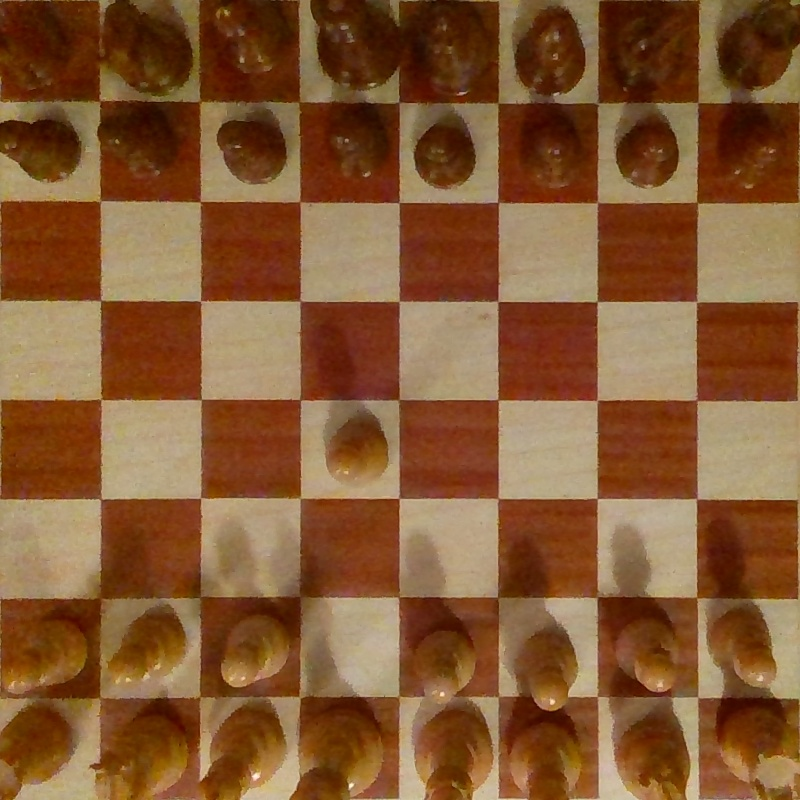
\includegraphics[width=0.18\textwidth]{segmented_board.jpg} & 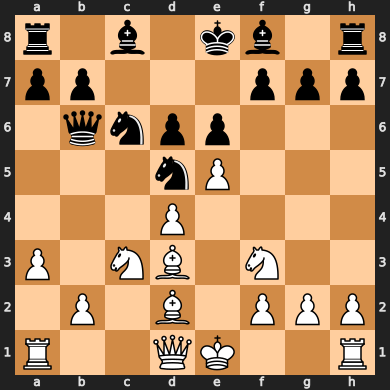
\includegraphics[width=0.18\textwidth]{fen.png} & 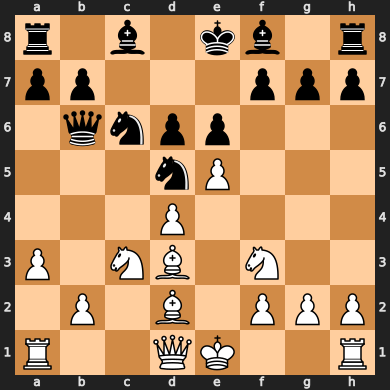
\includegraphics[width=0.18\textwidth]{fen.png} & 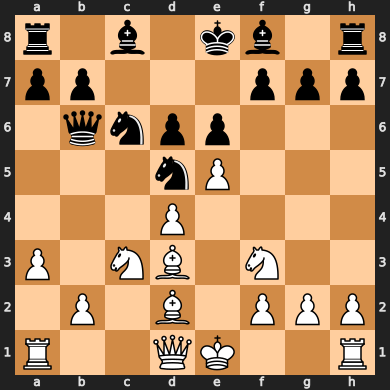
\includegraphics[width=0.18\textwidth]{fen.png} & 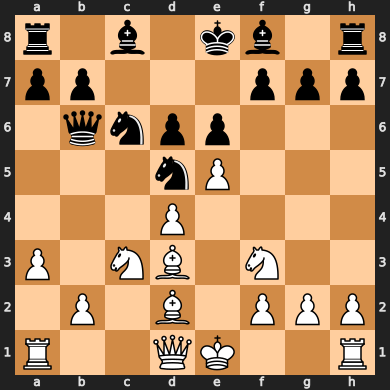
\includegraphics[width=0.18\textwidth]{fen.png} \\
    \hline
    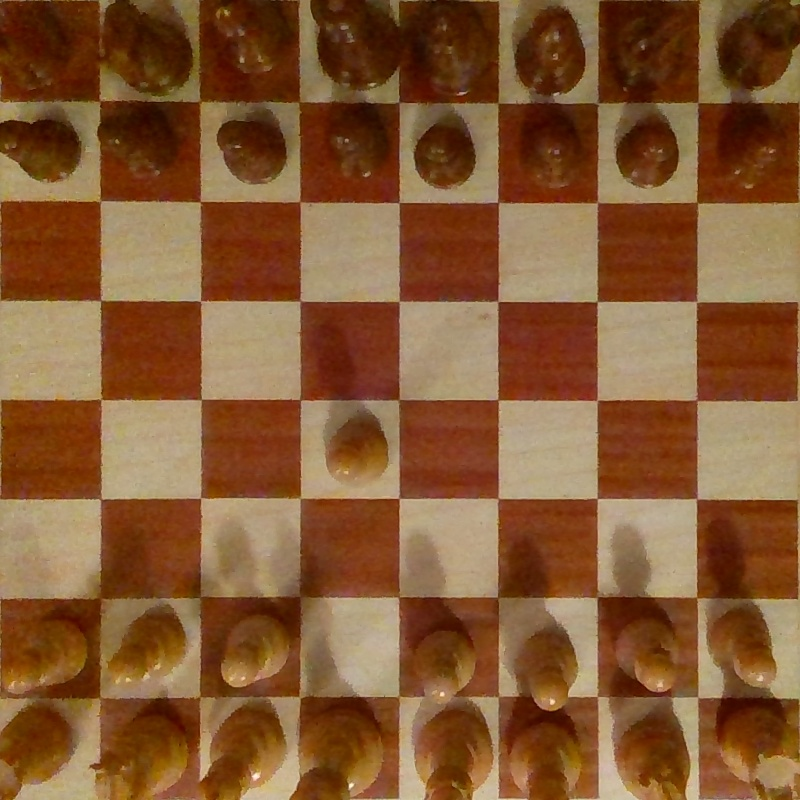
\includegraphics[width=0.18\textwidth]{segmented_board.jpg} & 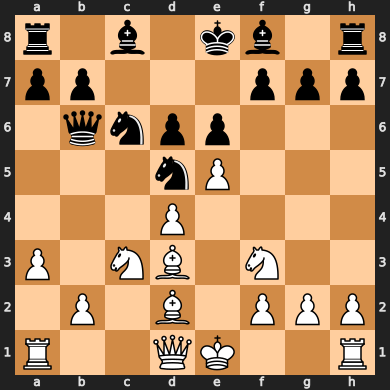
\includegraphics[width=0.18\textwidth]{fen.png} & 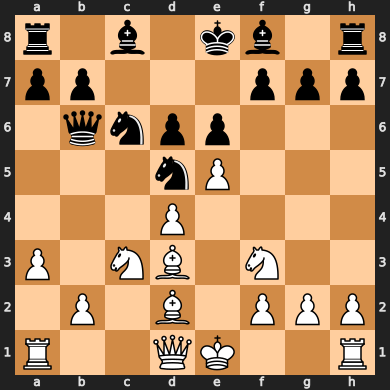
\includegraphics[width=0.18\textwidth]{fen.png} & 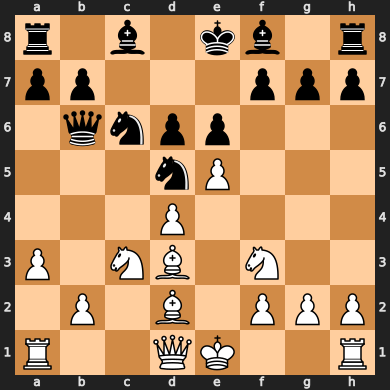
\includegraphics[width=0.18\textwidth]{fen.png} & 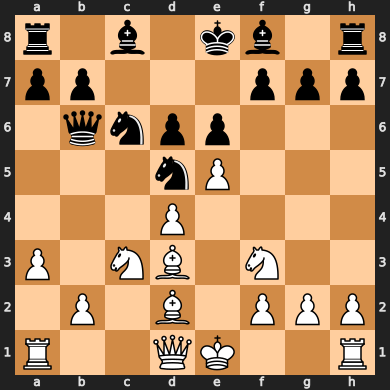
\includegraphics[width=0.18\textwidth]{fen.png} \\
    \hline
    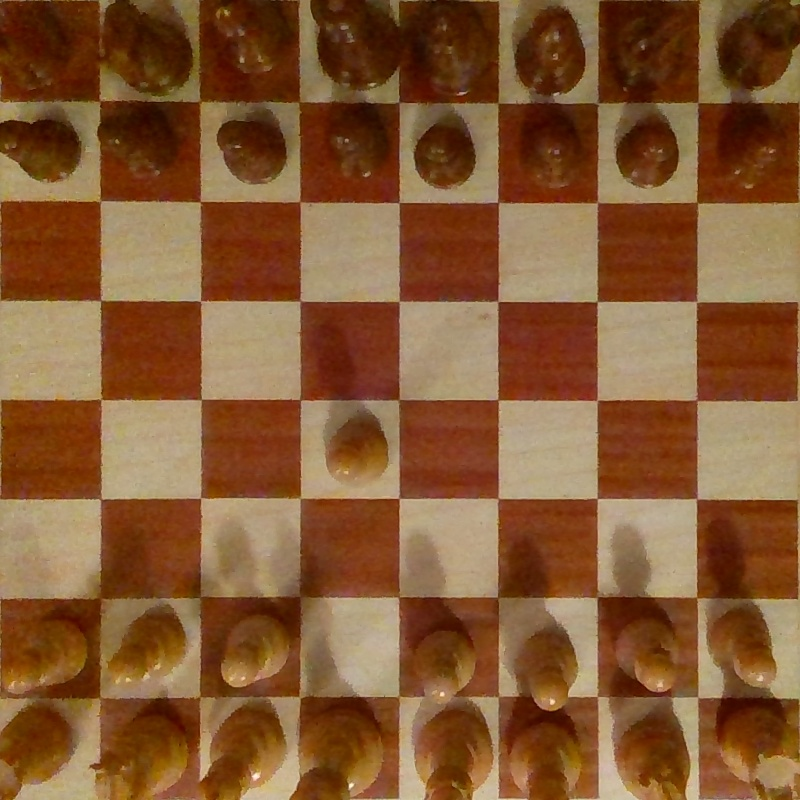
\includegraphics[width=0.18\textwidth]{segmented_board.jpg} & 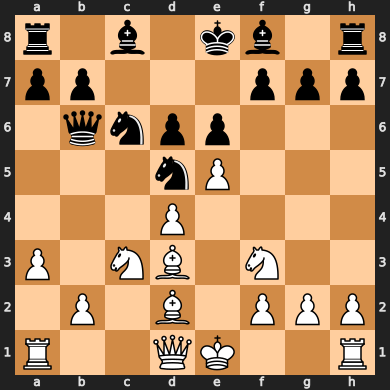
\includegraphics[width=0.18\textwidth]{fen.png} & 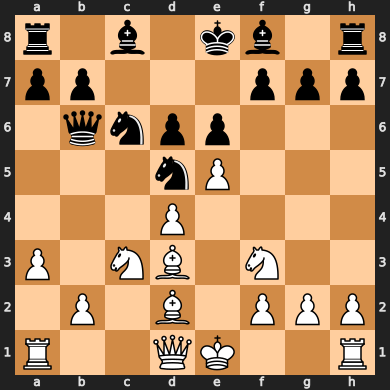
\includegraphics[width=0.18\textwidth]{fen.png} & 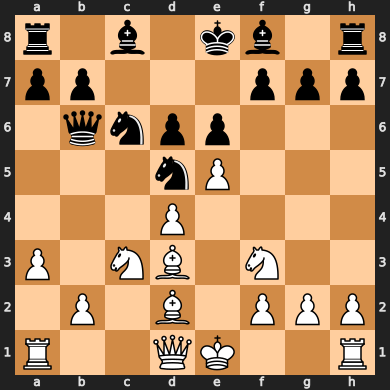
\includegraphics[width=0.18\textwidth]{fen.png} & 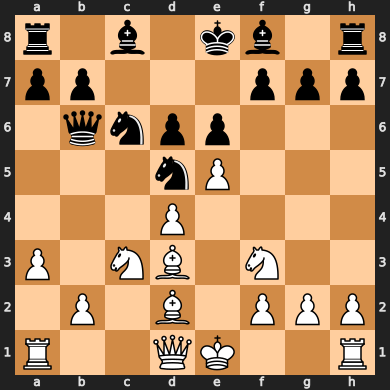
\includegraphics[width=0.18\textwidth]{fen.png} 
\end{tabu}}
\end{center}


Talk about speed of inference and any other limitations of both presented and other work.

\section{Recording PGN}
\label{evaluate pgn}
In addition to evalutaing the raw model's performance, six games of varying length are played from beginning to end 
with the inference application.  
How well does it perform.  What did it take to get there?

\begin{center}
\begin{tabular}{|c|c|c|c|}
    \hline
    Game & No. Moves & Mean Delay (100 ms) & PGN 100\% Correct \\
    \hline
    Kasparov 1 & 84 & 30 &  \checkmark \\
    Kasparov 2 & 43 & 32 & \checkmark \\
    Kasparov 3 & 47 & - & - \\
    Nakamura 4 & 122 & 25 & \checkmark \\
    \hline
\end{tabular}
\end{center}

How about performance?
Frames per second.  Analyse profiler.

\begin{figure}[h]
    \centering
    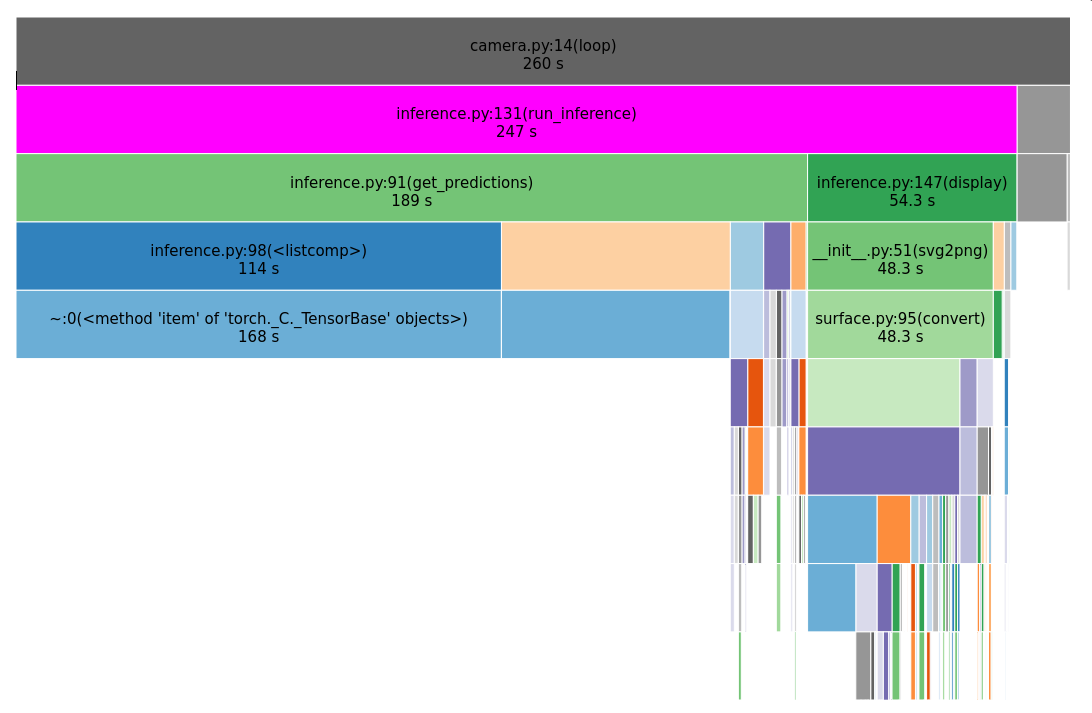
\includegraphics[width=\textwidth]{call_stack.png}
    \caption{cProfile Visualisation of recording a 4 minute game at inference with moves made in quick succession}
    \label{fig:profile}
\end{figure}